\clearpage

\begin{tcolorbox}	
\begin{tabular}{p{2.75cm} p{0.2cm} p{10.5cm}} 	
\textbf{Student Name}  &:& Tiago Esteves\\
\textbf{Starting Date} &:& October 03, 2017\\
\textbf{Goal}          &:& Implement the dimensioning of optical networks in the translucent transport mode.
\end{tabular}
\end{tcolorbox}

\section{Translucent with 1+1 Protection}
In this case study we focus on the translucent case with 1 + 1 protection.


\subsection{Physical Network Topology}

\subsubsection{Reference Network}
As we can see in the figure, our reference network consists of 6 nodes and 8 Bidirectional links.
The average length of the links was chosen so that the following calculations are more simplistic.

\begin{figure}[h!]
\centering
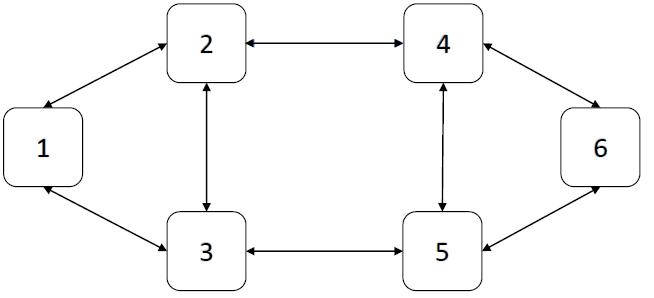
\includegraphics[width=\textwidth]{RedeTeste}
\caption{Physical Topology of the Reference Network.}
\end{figure}

The following table shows the values of the variables associated with this network.
\begin{table}[h!]
\centering
\begin{tabular}{|| c | c | c||}
 \hline
 Constant & Description & Value \\
 \hline\hline
 N & Number of Nodes & 6 \\
 L & Number of Bidirectional Links & 8 \\
 <$\delta$> & Node out-degree & 2,667 \\
 <len> & Mean Link Length (km) & 500 \\
 <h> & Mean Number of Hops,for Working Paths & 1,533 \\
 <h'> & Mean Number of Hops,for Backup Paths & 2,467 \\
 \hline
\end{tabular}
\caption{Table of reference network values}
\label{table:5}
\end{table}

As we can see from table \ref{table:5}, to do all the calculations necessary for this project, let us know the value of the traffic used. This value is defined depending on the scenario used, as we can see:
\begin{itemize}
  \item Low Traffic: \textbf{0.5 TBits/s}
  \item High Traffic: \textbf{5 TBits/s}
\end{itemize}

\subsubsection{Realistic Network}
The real network chosen for this work is the EON (European Optical Network).
The way the nodes are arranged geographically can be seen from the following figure.

\begin{figure}[h!]
\centering
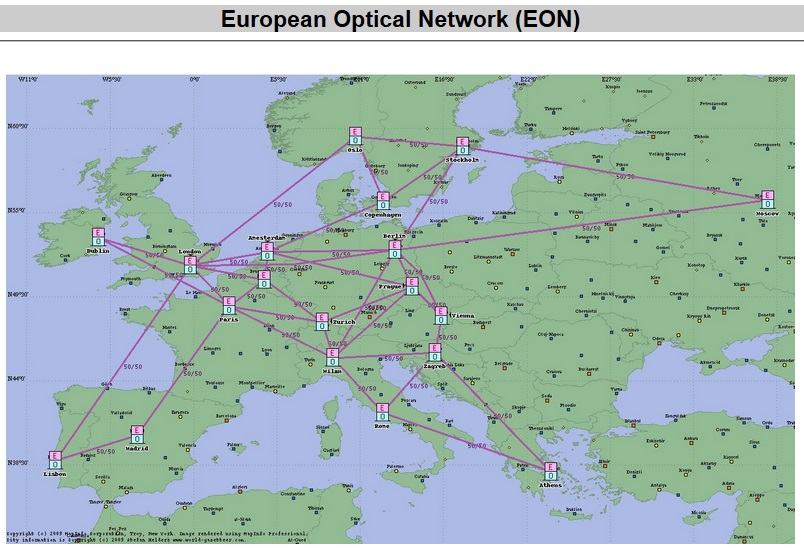
\includegraphics[width=\textwidth]{EON_Rede_Realista}
\caption{Physical Topology of the Realistic Network.}
\end{figure}

\begin{table}[h!]
The table \ref{table:6} shows the values of the variables associated with this network.\vspace{10pt}
\centering
\begin{tabular}{|| c | c | c||}
 \hline
 Constant & Description & Value \\
 \hline\hline
 N & Number of Nodes & 19 \\
 L & Number of Bidirectional Links & 37 \\
 <$\delta$> & Node out-degree & 3,89 \\
 <len> & Mean Link Length (km) & 753,76 \\
 <h> & Mean Number of Hops,for Working Paths & 2,3 \\
 <h'> & Mean Number of Hops,for Backup Paths & 3,2 \\
 \hline
\end{tabular}
\caption{Table of realistic network values}
\label{table:6}
\end{table}

Again, to make all the necessary calculations, only the value of the traffic used is missing. This value is set depending on the scenario used, as we can see:

\begin{itemize}
  \item Low Traffic: \textbf{2 TBits/s}
  \item High Traffic: \textbf{20 TBits/s}
\end{itemize}

\subsection{Dimensioning using ILP}

\subsubsection{ILP models}

\begin{equation}
minimize \qquad \qquad   \sum_{(p,k,b)} l[p,k,b]
\label{ILPTransluc}
\end{equation}

$subject$ $to$

\begin{equation}
\sum_{k \neq s} L[s,d,o,s,k] == traffic[o,s,d]
\qquad \qquad \qquad \qquad \qquad \qquad
\forall s,d,o : s < d
\label{ILPTransluc1}
\end{equation}

\begin{equation}
\sum_{k \neq p \ k \neq s} L[s,d,o,p,k] == \sum_{k\textbackslash \{p,d\}} L[s,d,o,k,p]
\qquad \qquad
\forall s,d,p,o : s < d : p \neq s : p \neq d
\label{ILPTransluc2}
\end{equation}

\begin{equation}
\sum_{k \neq d} L[s,d,o,k,d] == traffic[o,s,d]
\qquad \qquad \qquad \qquad \qquad \qquad
\forall s,d,o : s < d
\label{ILPTransluc3}
\end{equation}

\begin{equation}
\sum_{(s,d,o): s<d} (granularities[o] \times L[s,d,o,p,k]) \Leftarrow  \sum_{b} BD[b] \times l[p,k,b]
\qquad \qquad
\forall p,k 
\label{ILPTransluc4}
\end{equation}

\begin{equation}
L[s,d,o,p,k] \geq 0;
\qquad \qquad \qquad \qquad \qquad \qquad \qquad \qquad \qquad \qquad
\forall s,d,p,k,o : s < d
\label{ILPTransluc5}
\end{equation}

\begin{equation}
\sum_{j \neq p} y[p,k,p,j,b] \equiv l[p,k,b]
\qquad \qquad \qquad \qquad \qquad \qquad \qquad \qquad
\forall k,p,b
\label{ILPTransluc6}
\end{equation}

\begin{equation}
\sum_{j\neq i \ j\neq p} y[p,k,i,j,b] \equiv \sum_{j \neq i \ j \neq k} y[p,k,j,i,b]
\qquad \qquad \qquad \qquad
\forall k,p,i,b : i \neq k : i \neq p
\label{ILPTransluc7}
\end{equation}

\begin{equation}
\sum_{j \neq k} y[p,k,j,k,b] \equiv l[p,k,b]
\qquad \qquad \qquad \qquad \qquad \qquad \qquad \qquad
\forall k,p,b
\label{ILPTransluc8}
\end{equation}

\begin{equation}
\sum_{(p,k,b)} \left( y[p,k,i,j,b] + y[p,k,j,i,b]\right) \leq 80 \times C[i,j]
\qquad \qquad \qquad \qquad
\forall i,j : i < j
\label{ILPTransluc9}
\end{equation}

\begin{equation}
y[p,k,i,j,b] \geq 0
\qquad \qquad \qquad \qquad \qquad \qquad \qquad \qquad \qquad \qquad \qquad \qquad
\forall p,k,i,j,b
\label{ILPTransluc10}
\end{equation}	


\subsubsection{ILP Results}

In this initial phase the results will be presented using ILP to calculate the CAPEX of the reference network.

The value of the CAPEX of the network will be calculated based on the costs of the equipment present in the figure below.
\begin{figure}[h!]
  \centering
  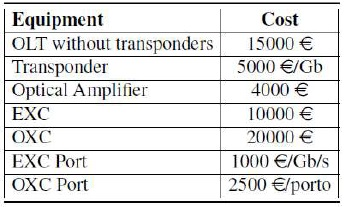
\includegraphics[scale=1]{TabValor}
  \caption{Table with costs}
\end{figure}

In addition to the equipment costs, we will also use the parameter "span", which in this case will have a value of 100.
Because this value is used to calculate the number of optical amplifiers required in the network using Equation \ref{amplifiersTranslu}.

\begin{equation}
N^R = \sum\limits_{l=1}^L\left(\left\lceil\frac{len_l}{span}\right\rceil-1\right)
\label{amplifiersTranslu}
\end{equation} \\

To know the value of CAPEX it is necessary to know the value of the cost of the links and the cost of the nodes.

To calculate the cost of the nodes, the sum of the costs of the optical and electrical node is made. %For this case the optical cost is given by equation \ref{opticalCost} and the electrical cost by the equation \ref{electricalCostTransp}.

%\begin{equation}
%C_{oxc} = \left(\gamma_{o0} \times N \right) + \gamma_{o1} \times  \left(P_{LINE} + P_{ADD}\right)
%\label{opticalCost}
%\end{equation}	
	
%\begin{itemize}
%\item{$C_{oxc}$		$\rightarrow$	Optical Ports Cost}
%\item{$\gamma_{o0}$	$\rightarrow$	OXC cost in Euros}
%\item{$\gamma_{o1}$	$\rightarrow$	OXC port cost in Euros}
%\item{$P_{TRIB}	$	$\rightarrow$	Number of tributary ports}
%\item{$P_{ADD} $	$\rightarrow$	Number of adding ports}
%\end{itemize}

%\begin{equation}
%C_{exc} = \left(\gamma_{e0}\times N\right) + \gamma_{e1} \times \left(2 \times T_1 \right)		\label{electricalCostTransp}
%\end{equation} \\


To calculate the cost of the Links we will use the equation .

%\begin{equation}
%C_L = \left(\gamma_0^{OLT} \times L\right) + \left(\gamma_1^{OLT} \times \tau \times W\right) + \left(N^R \times %c^R\right)
%\label{linkCostsTransp}
%\end{equation} \\
	

Finally we will calculate the CAPEX values for the various situations mentioned.\\

\textbf{Low Traffic scenario:}\\

$C_L$ = \textbf{\euro}

$C_N$ = \textbf{\euro}

$CAPEX$ = \textbf{\euro}\\

\textbf{High Traffic scenario:}\\

$C_L$ = \textbf{\euro}

$C_N$ = \textbf{ \euro}

$CAPEX$ =  \textbf{ \euro}\\



\subsection{Dimensioning using Heuristics}

\subsubsection{Heuristics Models}

\subsubsection{Heuristics Results}

\subsection{Analysis and comparison of results}
